\subsection{Neurons}
The term "\textbf{neural network}" is a reference to the workings of nervous systems of animals. These systems consist of a net of neurons, which are biological cells that are intricately connected to other neurons through structures called synapses. These connections carry electrical pulses between the different neurons that can excite them when they exceed certain thresholds. These thresholds vary from neuron to neuron and change over time. When this excitation occurs, new pulses in turn propagate from the excited neuron outwards to possibly excite other neurons. This interplay between excitation and transmission through the network of neurons is believed to be create what we perceive as thinking. Mathematical analyses of these systems in attempts to eventually understand and replicate this thinking process have been done as early as the 1940's.\cite{A_logical_calculus_of_the_ideas_immanent_in_nervous_activity}\\
The artificial neural networks that we use for machine learning are modern attempts to replicate parts of those biological networks. The neurons, which are the building bricks of the artificial neural networks, are mathematical entities that take a fixed number of scalar values as inputs and convert them into a single output value. For a more visual explanation let's take a look at \cref{fig:Neuron_explanation}.
\begin{figure}
	\centering
	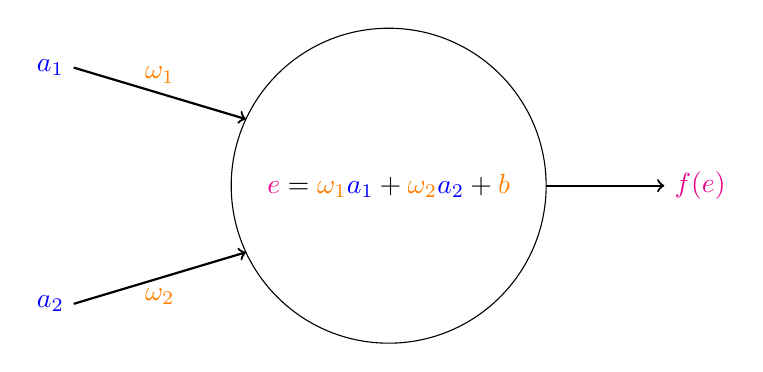
\begin{tikzpicture}[shift={(0,0)}]
	\draw (5,5) circle[radius=2];
	
	% Calculate the coordinates on the circle's circumference
	\pgfmathsetmacro\arrowOneX{5 + cos(155) * 2} % 45 degrees angle
	\pgfmathsetmacro\arrowOneY{5 + sin(155) * 2}
	
	\pgfmathsetmacro\arrowTwoX{5 + cos(-155) * 2} % 135 degrees angle
	\pgfmathsetmacro\arrowTwoY{5 + sin(-155) * 2}
		
	\draw[->, thick] (1,6.5) -- (\arrowOneX, \arrowOneY) node[pos=0.5,above] {$\textcolor{orange}{\omega_1}$};
	\draw (1,6.5) node[left] {$\textcolor{blue}{a_1}$};
	\draw[->, thick] (1,3.5) -- (\arrowTwoX, \arrowTwoY) node[pos=0.5,below] {$\textcolor{orange}{\omega_2}$};
	\draw (1,3.5) node[left] {$\textcolor{blue}{a_2}$};
	\node at (5,5) {$\textcolor{magenta}{e} = \textcolor{orange}{\omega_1}\textcolor{blue}{a_1} + \textcolor{orange}{\omega_2}\textcolor{blue}{a_2} + \textcolor{orange}{b}$};	
	\draw[->, thick] (7,5) -- (8.5,5) node[right] {$\textcolor{magenta}{f(e)}$};
	
	
\end{tikzpicture}
	\caption{This figure aids the explanation of the general operating principle of neurons in neural networks as they are used in this thesis. The parameters $\omega_i$ are denoted in orange, the input activations $a_i$ in blue and the activation $e$ with its corresponding activation function $f$ in violet.}
	\label{fig:Neuron_explanation}
\end{figure}
This is a case with two inputs. The big circle in the middle is representing the neuron itself. It takes as input the activation values $a_i$, multiplies them with their corresponding weights $\omega_i$, sums them up, adds a bias value $b$ and then applies the activation function to get the resulting output value. The input activations $a_i$ correspond to the electronic pulses in the nerve system, with the strength of the pulse coded into the value itself. No pulse in the biological system would be represented by an activation of zero in the mathematical model. The weights $\omega_i$ are a representation of how important single input values are for the activation of the neuron itself. In the biological counterpart this might correspond to how thick or conductive the connections between the nerve cells are. Finally, the combination of bias $b$ and activation function describes how high the sum of the input-weight-pairs has to be to activate the neuron and how the resulting value for the activation of the neuron changes for higher input activations. For example, a very simple output activation function would be a heaviside function ($f(x) = 1$ for $x\geq0$ and $f(x) = 0$ for $x<0$). The neuron then outputs $1$ if the sum of the input-weight-pairs is bigger than the negative bias $-b$, which results in a positive value for $e$ and $0$ otherwise. One could say that the neuron can only be on or off. A more common activation function that will be used for the rest of this thesis is the ReLU function (Rectified Linear Unit). This function is defined as 
\begin{equation}
	f(x) = 
	\begin{cases}
		x, &\text{if } x\geq0 \\
		0, &\text{otherwise}
	\end{cases}.
\end{equation}
Here the neuron gets activated as soon as the sum of the input-weight-pairs is higher than $-b$ and the value of the activation increases linearly with $e$ for those high sums.
\subsection{Neural networks}\label{sec:NeuralNetworks}
A neural network can be built from these neurons, by connecting the outputs of certain neurons to the inputs of others. For example lets take a look at \cref{fig:Neural_network_example}. This neural network consists of three layers of four neurons each, takes two values as input and outputs one value at the end. It could for example be trained for detecting if a point on a 2d-grid is inside or outside of a given region. The input values would be the $x$ and $y$ coordinates of the point and the output value could represent the probability of the point being inside the desired region. How exactly this training would work will be explained in later sections. \\
\begin{figure}
	\centering
	\begin{tikzpicture}
	\Vertex[x=0,y=0]{A}
	\Vertex[x=0,y=1]{B}
	\Vertex[x=0,y=2]{C}
	\Vertex[x=0,y=3]{D}
	
	\Vertex[x=2,y=0]{E}
	\Vertex[x=2,y=1]{F}
	\Vertex[x=2,y=2]{G}
	\Vertex[x=2,y=3]{H}
	
	\Vertex[x=4,y=0]{I}
	\Vertex[x=4,y=1]{J}
	\Vertex[x=4,y=2]{K}
	\Vertex[x=4,y=3]{L}
	
	\Edge[lw=1pt](A)(E)
	\Edge[lw=1pt](A)(F)
	\Edge[lw=1pt](A)(G)
	\Edge[lw=1pt](A)(H)
	
	\Edge[lw=1pt](B)(E)
	\Edge[lw=1pt](B)(F)
	\Edge[lw=1pt](B)(G)
	\Edge[lw=1pt](B)(H)
	
	\Edge[lw=1pt](C)(E)
	\Edge[lw=1pt](C)(F)
	\Edge[lw=1pt](C)(G)
	\Edge[lw=1pt](C)(H)
	
	\Edge[lw=1pt](D)(E)
	\Edge[lw=1pt](D)(F)
	\Edge[lw=1pt](D)(G)
	\Edge[lw=1pt](D)(H)
	
	\Edge[lw=1pt](E)(I)
	\Edge[lw=1pt](E)(J)
	\Edge[lw=1pt](E)(K)
	\Edge[lw=1pt](E)(L)
	
	\Edge[lw=1pt](F)(I)
	\Edge[lw=1pt](F)(J)
	\Edge[lw=1pt](F)(K)
	\Edge[lw=1pt](F)(L)
	
	\Edge[lw=1pt](G)(I)
	\Edge[lw=1pt](G)(J)
	\Edge[lw=1pt](G)(K)
	\Edge[lw=1pt](G)(L)
	
	\Edge[lw=1pt](H)(I)
	\Edge[lw=1pt](H)(J)
	\Edge[lw=1pt](H)(K)
	\Edge[lw=1pt](H)(L)
	
	\Vertex[x=-2,y=1, label=$x$, opacity = 0]{X}
	\Vertex[x=-2,y=2, label=$y$, opacity = 0]{Y}
	\Edge[lw=1pt](X)(A)
	\Edge[lw=1pt](X)(B)
	\Edge[lw=1pt](X)(C)
	\Edge[lw=1pt](X)(D)
	\Edge[lw=1pt](Y)(A)
	\Edge[lw=1pt](Y)(B)
	\Edge[lw=1pt](Y)(C)
	\Edge[lw=1pt](Y)(D)
	
	\Vertex[x=6,y=1.5, label=$p$, opacity = 1]{P}
	\Edge[lw=1pt](I)(P)
	\Edge[lw=1pt](J)(P)
	\Edge[lw=1pt](K)(P)
	\Edge[lw=1pt](L)(P)
	
	\draw [decorate,
	decoration = {brace, mirror, amplitude=10pt}] (-0.2,-0.5) --  (4.2,-0.5);
	\node at (2,-1.2) {3 (hidden) layers};
	\draw [decorate,
	decoration = {brace, mirror, amplitude=10pt}] (6.5,-0.3) --  (6.5,3.3);
	\node at (7.2,1.5) [rotate=-90] {width of 4 neurons};
	
\end{tikzpicture}
	\caption{This figure shows an example of a neural network. It consists of multiple neurons connected to each other. This specific network has 2 input values and one output value and a width of 4 neurons for a total of 3 layers. The names of those input and output values correspond to the use case of identifying if a 2d point lies within a region in 2d space.}
	\label{fig:Neural_network_example}
\end{figure}
This network is only a very specific example of what a neural network might look like. In reality, there are various kinds of networks used to learn different tasks. For this thesis we will only talk about "fully connected" or "dense" neural networks. This means that every neuron in the first layer will receive every possible input value, and every neuron in later layers will receive the output of every neuron in the previous layer as an input. The activation function is the same for every neuron in this case, but the weights and biases vary throughout. How the output of the network gets handled may still differ through different use cases. Most of the time, the output is generated by regular neurons and gets fed into a softmax at the end. Details on the softmax function can be found in \cite{gao2018properties}. For our understanding it's enough to know that the softmax function converts the values of the output nodes into probabilities that add up to $1$, where a higher value results in a higher corresponding probability. The structure of a neural network is generally called the architecture of the network, with the hidden layers or simply layers referring to the columns of neurons in between the input values and output neurons and the amount of neurons per layer referred to as the "width" of the network. This is also denoted in \cref{fig:Neural_network_example}. 
\subsection{Mathematical view}
The previous explanations have been very visual and step by step in an attempt to make the topic more accessible. However, these concepts can be broken down to rather short mathematical expressions.\\
To start off we can define the inputs as $a_i^{(0)}$ , $i =  1, \dotsb n$, with $n$ being the amount of inputs. The weights of the first hidden layer can be denoted by $\omega_{i}^{(1)}$, $i =  1, \dotsb n$. Further we define $\omega_{i,j}^{(k)}$ as the weight that connects the $i$-th neuron in the $k$-th layer with the $j$-th neuron in the $(k-1)$-th layer. The values that $i$ and $j$ can assume depend on the widths of the respective layers, $k$ can reach values between $1$ and the amount of hidden layers plus 1, for the output layer. The bias of the $i$-th neuron in the $k$-th layer is denoted as $b_i^{(k)}$. Using this notation we can instantly write out the output of the $i$-th neuron in the $k+1$-th layer as
\begin{equation}
	a_i^{(k+1)} = f\left(\sum_j \left(\omega_{i,j}^{(k+1)}a_j^{(k)}\right) + b_i^{(k+1)}\right).
\end{equation}
To actually calculate the value, the $a_j^{(k)}$ values have to be recursively replaced with their full calculation until one arrives at the input values of the network.\\
For simplicity reasons we will refer to the weights $\omega_{i,j}^{(k)}$ and biases $b_i^{(k)}$ together as "parameters" of the neural network. We will denote these collected in one ordered set as $\theta = \{\theta_i\}_{i=1}^{N}$ if $N$ is the amount of weights and the amount of biases added together. The mapping of the parameters onto $\theta$ is not important as long as it is known so that one can calculate the output of a neural network if given $\theta$ in the same way as when one is given the parameters. Another possible representation that we will use often is to write this set as a vector $\theta \in \mathbb{R}^N$. A short notation for the output of the neural network will be explained in the next section.
